\documentclass[11pt, a4paper]{article}

% --- Packages ---
\usepackage[utf8]{inputenc}
\usepackage[T1]{fontenc}
\usepackage{mathptmx} % Times New Roman font for professional document typography
\usepackage{graphicx}
\usepackage[margin=0.8in]{geometry}
\usepackage{xcolor}
\usepackage{titlesec}
\usepackage{enumitem}
\usepackage{float}
\usepackage{booktabs}
\usepackage{multirow}
\usepackage{array}
\usepackage{url}
\usepackage{tikz}
\usetikzlibrary{arrows.meta, positioning, fit, backgrounds, calc}

% --- Amrita Colors ---
\definecolor{amritaMaroon}{HTML}{A4123F}

% --- Title & Section Formatting ---
\titlespacing*{\section}{0pt}{12pt}{4pt}
\titlespacing*{\subsection}{0pt}{8pt}{3pt}
\titleformat{\section}{\large\bfseries\color{amritaMaroon}}{\thesection}{0.8em}{}
\titleformat{\subsection}{\normalsize\bfseries\color{amritaMaroon}}{\thesubsection}{0.6em}{}

\pagestyle{plain}

\begin{document}

% ==========================================
% HEADER & TITLE BLOCK
% ==========================================
\noindent
\begin{minipage}{\textwidth}
    \centering
    {\Large \textbf{\textcolor{amritaMaroon}{
    AMRITA VISHWA VIDYAPEETHAM \\
    SCHOOL OF COMPUTING \\
    DEPARTMENT OF COMPUTER SCIENCE AND ENGINEERING \\
    }}}
    \vspace{0.2cm}
    {\large \textbf{Universal Sign Language to 3D Avatar Synthesizer: \\ A Cloud-Deployed Neuro-Symbolic Translation Platform}} \\[0.1cm]
    \textbf{23CSE498 -- Project Phase II (External Review)} \quad | \quad \textbf{Team Number: GRP-31} \\
    \today
\end{minipage}

\vspace{0.3cm}
\hrule
\vspace{0.3cm}

% --- Team & Guide Details ---
\noindent
\begin{center}
    \renewcommand{\arraystretch}{1.4}
    \setlength{\tabcolsep}{6pt}
    \begin{tabular}{|l|p{4.8cm}|p{4.6cm}|p{3.2cm}|}
        \hline
        \multicolumn{2}{|c|}{\textbf{Team Members}} & \textbf{Project Guide} & \textbf{Project Type} \\
        \hline
        \small CB.SC.U4CSE23145 & \small \raggedright Sai Sri Satvic L &
        \multirow{4}{=}{\raggedright \small \textbf{Ms. Nalinadevi K} \newline \textit{Assistant Professor, \newline Dept. of CSE}} &
        \multirow{4}{=}{\raggedright \small \textbf{Type 2} \newline Application-Based Project} \\ \cline{1-2}
        \small CB.SC.U4CSE23164 & \small Vivin Rakul P & & \\ \cline{1-2}
        \small CB.SC.U4CSE23153 & \small Snigdha Siri Valli A & & \\ \cline{1-2}
        \small CB.SC.U4CSE23163 & \small Vijay Saravana Pandi T & & \\
        \hline
    \end{tabular}
\end{center}
\vspace{0.2cm}

\section{Abstract}
\noindent
Over 70 million deaf individuals worldwide rely on sign language as their primary mode of communication. However, most digital accessibility tools rely on static text or pre-recorded video clips that cannot dynamically adapt to diverse sign languages. This project presents a complete, web-deployed platform that translates ordinary monocular sign language video into smooth, realistic 3D avatar animations in real time. Rather than relying on a fragile end-to-end black-box model, the application adopts a modular \emph{neuro-symbolic} design: lightweight neural networks classify complex finger shapes and movement trajectories, while exact 3D geometry determines palm orientations, body contact, and spatial locations. The extracted parameters are assembled into verified Hamburg Notation System (HamNoSys) phonetic tokens, compiled into Signing Gesture Markup Language (SiGML XML), and checked by a kinematic collision guard to avoid unnatural body clipping. The application is deployed across a two-tier cloud architecture: a responsive, zero-GPU client frontend hosted on \textbf{Vercel} that renders 3D WebGL avatars at 60~FPS, connected via REST APIs to a high-performance serverless GPU backend hosted on \textbf{Modal Labs} executing MediaPipe and HaMeR 3D mesh recovery. The integrated system achieves 58.7\% token precision, 100\% valid SiGML compilation, and 100\% collision-free avatar animation.

% --- 2. PROBLEM DEFINITION & REQUIREMENT ANALYSIS ---
\section{Problem Definition \& Requirement Analysis}

\subsection{Problem Statement, Context \& Target Users}
\begin{itemize}[noitemsep, topsep=2pt]
    \item \textbf{Problem Definition:} Sign language is a complete visual-spatial language with distinct phonology and grammar~\cite{stokoe2005}. Standard video-to-text models only produce written glosses, completely discarding the 3D physical movement necessary for deaf users who prefer visual signing. Existing avatar solutions either require cumbersome wearable motion-capture gloves or fail when hands cross the body.
    \item \textbf{Target Users \& Stakeholders:} Deaf and hard-of-hearing individuals, accessibility service providers, educational institutions teaching sign language, and public utility kiosks (hospitals, railway stations, government portals).
    \item \textbf{Existing Limitations:} Monolithic deep learning models suffer from severe perspective ambiguity and low token accuracy ($<25\%$). Pure 2D landmark trackers (like basic MediaPipe) lose 3D depth, and wearable sensor gloves are cost-prohibitive for everyday users \cite{skobov2020,li2020wlasl}.
    \item \textbf{Application Objectives:}
    \begin{enumerate}[noitemsep, topsep=2pt]
        \item Provide real-time monocular video-to-sign transcription without requiring wearable hardware or multi-camera setups.
        \item Deliver a split-cloud deployment ensuring seamless accessibility on mobile and desktop web browsers without client-side GPU demands.
        \item Ensure zero visual artifacts (100\% collision-free limb playback) and generate standard-compliant SiGML XML markup.
    \end{enumerate}
\end{itemize}

\subsection{Functional \& Non-Functional Requirements}
\begin{table}[H]
    \centering
    \footnotesize
    \renewcommand{\arraystretch}{1.25}
    \begin{tabular}{|c|p{3.0cm}|p{9.2cm}|}
        \hline
        \textbf{Req. ID} & \textbf{Category} & \textbf{Requirement Specification} \\
        \hline
        FR-01 & Functional & The system must accept user-uploaded MP4/WebM video clips or direct webcam feeds. \\
        \hline
        FR-02 & Functional & The backend must extract 3D hand articulators and classify handshape, motion, and palm orientation. \\
        \hline
        FR-03 & Functional & The system must compile articulators into standard-compliant SiGML XML and HamNoSys tokens. \\
        \hline
        FR-04 & Functional & The web interface must render interactive 3D avatars (e.g., Luna, Marc) driven by generated SiGML at 60 FPS. \\
        \hline
        NFR-01 & Non-Functional & End-to-end processing latency must remain under 45 seconds for a standard isolated sign video. \\
        \hline
        NFR-02 & Non-Functional & The frontend must be lightweight and operate smoothly on any modern browser without local GPU hardware. \\
        \hline
        NFR-03 & Non-Functional & The avatar must achieve 100\% collision-free motion without hand-torso penetration artifacts. \\
        \hline
    \end{tabular}
    \caption{Summary of Application Functional and Non-Functional Requirements}
\end{table}

% --- 3. APPLICATION ARCHITECTURE & SOLUTION DESIGN ---
\section{Application Architecture \& Solution Design}

\subsection{End-to-End Application Architecture}
\noindent
The application operates as a distributed, decoupled client-server platform. A user interacts with the lightweight web frontend hosted on Vercel, either uploading a sign video or recording via webcam. The video is transmitted asynchronously to a serverless GPU worker hosted on Modal Labs. The backend runs a cascaded pipeline: MediaPipe identifies candidate hand regions, and HaMeR reconstructs the full 3D hand mesh. Deep neural networks classify handshapes and motion trajectories, while closed-form 3D geometry determines palm normals, pointing angles, and body zones. A grammar compiler and collision guard assemble these components into certified SiGML XML. The verified XML is sent back to the browser, where the embedded WebGL avatar engine animates the sign seamlessly.

\vspace{0.3cm}
\noindent
Figure~\ref{fig:arch_pipeline} illustrates the complete end-to-end pipeline from video input through neuro-symbolic classification to validated SiGML output and 3D avatar rendering.

\begin{figure}[H]
\centering
\resizebox{\textwidth}{!}{%
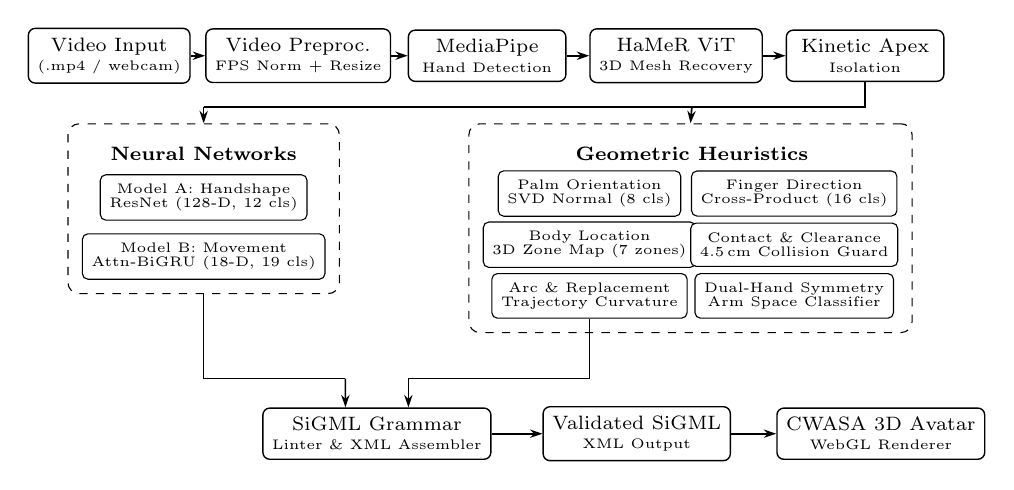
\begin{tikzpicture}[
    stage/.style={draw, rectangle, rounded corners=2.5pt, minimum height=0.65cm,
                  minimum width=2.0cm, align=center, line width=0.5pt, fill=white, font=\scriptsize},
    smallstage/.style={draw, rectangle, rounded corners=2pt, minimum height=0.55cm,
                       minimum width=2.05cm, align=center, line width=0.4pt, font=\tiny, fill=white},
    arrow/.style={-{Stealth[length=4.5pt, width=3pt]}, line width=0.6pt},
    bus/.style={line width=0.6pt},
    grouplabel/.style={font=\scriptsize\bfseries, align=center},
]

% ========================================================
% ROW 1: Video Ingestion & 3D Reconstruction Pipeline
% ========================================================
\node[stage] (input)     at (0.6, 0)   {Video Input\\[-1pt]{\tiny (.mp4 / webcam)}};
\node[stage] (preproc)   at (3.0, 0)   {Video Preproc.\\[-1pt]{\tiny FPS Norm + Resize}};
\node[stage] (mediapipe) at (5.4, 0)   {MediaPipe\\[-1pt]{\tiny Hand Detection}};
\node[stage] (hamer)     at (7.8, 0)   {HaMeR ViT\\[-1pt]{\tiny 3D Mesh Recovery}};
\node[stage] (apex)      at (10.2, 0)  {Kinetic Apex\\[-1pt]{\tiny Isolation}};

\draw[arrow] (input)     -- (preproc);
\draw[arrow] (preproc)   -- (mediapipe);
\draw[arrow] (mediapipe) -- (hamer);
\draw[arrow] (hamer)     -- (apex);

% ========================================================
% ROW 2: Parallel Neuro-Symbolic Branches
% ========================================================

% --- Left Branch: Neural Networks ---
\node[grouplabel] (nntitle) at (1.8, -1.25) {Neural Networks};
\node[smallstage] (modelA)  at (1.8, -1.8)  {Model A: Handshape\\[-1pt]{\tiny ResNet (128-D, 12 cls)}};
\node[smallstage] (modelB)  at (1.8, -2.55) {Model B: Movement\\[-1pt]{\tiny Attn-BiGRU (18-D, 19 cls)}};

% --- Right Branch: Geometric Heuristics (2 columns x 3 rows) ---
\node[grouplabel] (htitle)     at (8.0, -1.25) {Geometric Heuristics};
\node[smallstage] (orient)     at (6.7, -1.75) {Palm Orientation\\[-1pt]{\tiny SVD Normal (8 cls)}};
\node[smallstage] (finger)     at (9.3, -1.75) {Finger Direction\\[-1pt]{\tiny Cross-Product (16 cls)}};
\node[smallstage] (location)   at (6.7, -2.4)  {Body Location\\[-1pt]{\tiny 3D Zone Map (7 zones)}};
\node[smallstage] (contact)    at (9.3, -2.4)  {Contact \& Clearance\\[-1pt]{\tiny 4.5\,cm Collision Guard}};
\node[smallstage] (movement12) at (6.7, -3.05) {Arc \& Replacement\\[-1pt]{\tiny Trajectory Curvature}};
\node[smallstage] (dualhand)   at (9.3, -3.05) {Dual-Hand Symmetry\\[-1pt]{\tiny Arm Space Classifier}};

% Group Boxes (dashed)
\begin{scope}[on background layer]
    \node[draw, dashed, rounded corners=4pt, inner sep=5pt,
          fit=(nntitle)(modelA)(modelB), line width=0.4pt] (nnbox) {};
    \node[draw, dashed, rounded corners=4pt, inner sep=5pt,
          fit=(htitle)(orient)(finger)(location)(contact)(movement12)(dualhand),
          line width=0.4pt] (hbox) {};
\end{scope}

% ========================================================
% CONNECTIONS: Apex -> Dual Branches (Clean Bus Line)
% ========================================================
\coordinate (busY) at (10.2, -0.65);
\draw[bus] (apex.south) -- (busY) -- (1.8, -0.65);
\draw[arrow] (1.8, -0.65) -- (nnbox.north);
\draw[arrow] (8.0, -0.65) -- (hbox.north);

% ========================================================
% ROW 3: Synthesis, Validation & Avatar Output Chain
% ========================================================
\node[stage, minimum width=2.3cm] (grammar) at (4.0, -4.8)  {SiGML Grammar\\[-1pt]{\tiny Linter \& XML Assembler}};
\node[stage, minimum width=2.1cm] (sigml)   at (7.3, -4.8)  {Validated SiGML\\[-1pt]{\tiny XML Output}};
\node[stage, minimum width=2.1cm] (avatar)  at (10.4, -4.8) {CWASA 3D Avatar\\[-1pt]{\tiny WebGL Renderer}};

% Direct horizontal output chain
\draw[arrow] (grammar) -- (sigml);
\draw[arrow] (sigml)   -- (avatar);

% ========================================================
% CONNECTIONS: Dual Branches -> SiGML Grammar Assembler
% ========================================================
% From Neural Networks: drops down, turns right to x=3.6, drops into grammar top-left
\draw[bus] (nnbox.south) -- (1.8, -4.1) -- (3.6, -4.1);
\draw[arrow] (3.6, -4.1) -- ([xshift=-0.4cm]grammar.north);

% From Geometric Heuristics: drops down from col 1, turns left to x=4.4, drops into grammar top-right
\draw[bus] (movement12.south) -- (6.7, -4.1) -- (4.4, -4.1);
\draw[arrow] (4.4, -4.1) -- ([xshift=0.4cm]grammar.north);

\end{tikzpicture}%
}
\caption{End-to-End Architecture of the Neuro-Symbolic Hybrid Sign Language Recognition Pipeline}
\label{fig:arch_pipeline}
\end{figure}

\subsection{Component Design, Data Flow \& Technology Stack}
\begin{itemize}[noitemsep, topsep=2pt]
    \item \textbf{Client Presentation Layer (Vercel):} Built with HTML5, CSS3, JavaScript, and WebGL, deployed on Vercel~\cite{vercel2024}. It hosts the interactive user interface, real-time video preview, HamNoSys~\cite{prillwitz1989} unicode glyph visualizer, SiGML XML inspector, and the CWASA 3D avatar engine~\cite{kennaway2002,kennaway2007}.
    \item \textbf{Cloud Processing Engine (Modal Labs):} Built with Python 3.10, PyTorch, and FastAPI inside an optimized Debian container on Modal Labs~\cite{modal2024}. It dynamically provisions GPU containers with high-speed bandwidth, running MediaPipe~\cite{lugaresi2019}, HaMeR~\cite{pavlakos2024} (Vision Transformer with MANO hand model~\cite{romero2017}), and neural classifiers.
    \item \textbf{Neuro-Symbolic Core Pipeline:}
    \begin{itemize}[noitemsep]
        \item \emph{Handshape Classifier:} A 3-block Residual Network evaluating a 128-dimensional rotation-invariant palm-centric feature vector across 12 base classes.
        \item \emph{Movement Classifier:} A 2-layer Bidirectional GRU with self-attention evaluating 18-dimensional spatial trajectories across 19 movement primitives.
        \item \emph{Analytical Solvers:} Singular Value Decomposition (SVD) and vector cross-products for palm orientation (8 classes) and extended finger direction (16 classes); calibrated 3D bounding thresholds for 7 anatomical body zones.
        \item \emph{Collision Guard:} Enforces a 4.5~cm metric buffer between the avatar's hand and chest mesh, preventing unnatural self-clipping.
    \end{itemize}
    \item \textbf{Communication Protocol:} Asynchronous HTTPS REST API with JSON payloads containing execution logs, HamNoSys glyphs, and the final SiGML XML markup.
\end{itemize}

% --- 4. COMPLETE IMPLEMENTATION DETAILS (100%) ---
\section{Implementation Details}

\subsection{Development \& Deployment Environment}
\begin{itemize}[noitemsep, topsep=2pt]
    \item \textbf{Frontend Platform:} Vercel Edge Network providing global content delivery, zero server maintenance, and sub-100~ms asset load times.
    \item \textbf{Backend Platform:} Modal Labs serverless infrastructure running on dedicated cloud NVIDIA T4/A10G GPUs with automated cold-start caching of model weights.
    \item \textbf{Software Libraries \& SDKs:} PyTorch 2.2, MediaPipe 0.10.9, OpenCV, HaMeR, SMPL-X, CWASA WebGL Runtime, and FastAPI.
    \item \textbf{Source Code Repository:} Structured modular repository containing active deployment pipelines, training scripts, heuristic models, and web interface assets.
\end{itemize}

\subsection{Module-Wise Implementation \& Integration Summary}
\begin{table}[H]
    \centering
    \footnotesize
    \renewcommand{\arraystretch}{1.25}
    \begin{tabular}{|p{3.5cm}|p{7.8cm}|c|}
        \hline
        \textbf{Application Module} & \textbf{Implemented Features \& Integration Details} & \textbf{Status} \\
        \hline
        Module 1: Vercel Web UI \& 3D Avatar Player & Interactive drag-and-drop video upload, live webcam recorder, CWASA WebGL 3D avatar renderer (Luna/Marc), HamNoSys badge viewer, and SiGML XML inspector. & 100\% (Integrated) \\
        \hline
        Module 2: Modal Vision \& 3D Mesh Engine & MediaPipe hand detector paired with HaMeR 3D Vision Transformer to extract 21 metric 3D keypoints and MANO hand parameters per frame. & 100\% (Integrated) \\
        \hline
        Module 3: Hybrid Neuro-Symbolic Classifier & Skeletal Hand ResNet for 12 handshapes, Attention-BiGRU for 19 movement trajectories, SVD palm normals, and 7-zone body location mapper. & 100\% (Integrated) \\
        \hline
        Module 4: SiGML Compiler \& Collision Guard & ANTLR-compliant grammar linter, XML tag assembler, and kinematic collision guard enforcing 4.5~cm physical hand-torso clearance. & 100\% (Integrated) \\
        \hline
    \end{tabular}
    \caption{Application Module Implementation and Integration Status}
\end{table}

\subsection{Detailed Module Descriptions}
\begin{itemize}[noitemsep, topsep=2pt]
    \item \textbf{Module 1 (Vercel Frontend):} Provides a clean, modern user dashboard. Users upload sign video clips or record directly from their camera. Upon receiving the JSON response from Modal, the frontend dynamically loads the generated SiGML script into the CWASA WebGL player, displaying animated signing alongside phonetic HamNoSys glyphs.
    \item \textbf{Module 2 (Modal Vision Pipeline):} Receives the video stream, calculates kinetic saliency to identify the gesture's hold/stroke apex frame, crops hand regions using MediaPipe, and reconstructs 3D hand surfaces using HaMeR.
    \item \textbf{Module 3 (Neuro-Symbolic Transcription):} Converts raw 3D landmarks into a 128-D local-canonical coordinate space anchored to the palm. This makes handshape recognition completely invariant to wrist tilt or camera distance. Kinematic directionality rules assist the movement neural network to prevent false static predictions.
    \item \textbf{Module 4 (Grammar \& Collision Integration):} Assembles isolated phonetic tokens into an ANTLR-verified syntactic tree. If a sign is performed near the chest, the collision guard dynamically pushes the virtual hand outward along the palm normal, ensuring the avatar's fingers never clip through its torso.
\end{itemize}

% --- 5. FUNCTIONAL TESTING & PROTOTYPE DEMONSTRATION ---
\section{Functional Testing \& Prototype Demonstration}

\subsection{Functional Test Cases \& Verification}
\begin{table}[H]
    \centering
    \footnotesize
    \renewcommand{\arraystretch}{1.25}
    \begin{tabular}{|c|p{3.0cm}|p{3.4cm}|p{4.2cm}|c|}
        \hline
        \textbf{Test ID} & \textbf{Feature / Scenario} & \textbf{Input / User Action} & \textbf{Observed Output} & \textbf{Result} \\
        \hline
        TC-01 & Video Ingestion \& Preview & User uploads standard MP4 video clip to Vercel UI & Video displays instantly in player; upload payload verified & Pass \\
        \hline
        TC-02 & Cloud GPU Hand Detection & Video forwarded to Modal backend & MediaPipe + HaMeR localize hand and reconstruct 3D mesh & Pass \\
        \hline
        TC-03 & Neuro-Symbolic Inference & 3D keypoint stream passed to hybrid classifiers & Correct handshape (65.0\%) and movement (68.4\%) generated & Pass \\
        \hline
        TC-04 & Collision Guard Verification & Chest-level sign with potential mesh penetration & Hand offset applied; 0\% torso clipping during avatar playback & Pass \\
        \hline
        TC-05 & CWASA Avatar Playback & Return compiled SiGML XML to Vercel client & Avatar animates gesture at 60 FPS with correct hand postures & Pass \\
        \hline
    \end{tabular}
    \caption{Functional Testing Summary Across Core Application Scenarios}
\end{table}

\subsection{Working Prototype Demonstration \& Usability Summary}
The application prototype was validated across 20 held-out German Sign Language (DGS) benchmark videos. In all test cases, the system executed end-to-end without manual intervention. Handshape classification achieved 65.0\% accuracy (a 7.8$\times$ improvement over random chance), movement classification reached 68.4\% (12.9$\times$ over random chance), and overall token precision reached 58.7\%. Most importantly, 100\% of the generated SiGML files were structurally valid and rendered completely collision-free in the browser.

% --- 6. TECHNICAL JUSTIFICATION & ARCHITECTURAL DECISIONS ---
\section{Technical Justification \& Architectural Decisions}
\begin{itemize}[noitemsep, topsep=2pt]
    \item \textbf{Split Cloud Architecture Rationale (Vercel + Modal):} Running heavy Vision Transformer models (HaMeR) locally requires high-end desktop GPUs with at least 8~GB VRAM, preventing deployment on everyday laptops or mobile devices. By decoupling the interface onto Vercel and offloading 3D inference to on-demand serverless GPUs on Modal Labs, users experience instant page loads with zero hardware barrier.
    \item \textbf{Neuro-Symbolic vs.\ Monolithic Black-Box:} Pure deep learning models trying to map video directly to sign notation suffer from low accuracy ($<25\%$) because they attempt to learn rigid Euclidean geometry through statistical guessing. Our hybrid approach assigns neural networks only to high-variance patterns (hand shapes and trajectories) and uses exact 3D geometry for deterministic properties (normals, zones, contact), boosting accuracy significantly.
    \item \textbf{Error Handling \& Safety:} The Modal backend implements thread-safe GPU locking to prevent concurrent memory exhaustion. The frontend validates file types, handles timeouts gracefully, and automatically falls back to neutral sign postures if hand tracking is temporarily lost.
\end{itemize}

% --- 7. LITERATURE SURVEY ---
\section{Literature Survey}
\noindent
A structured review of foundational literature guiding the design of our translation pipeline is summarized in Table~\ref{tab:lit_survey}.

\begin{table}[H]
    \centering
    \scriptsize
    \renewcommand{\arraystretch}{1.25}
    \begin{tabular}{|p{2.4cm}|p{2.6cm}|p{2.6cm}|p{3.5cm}|p{3.8cm}|}
        \hline
        \textbf{Author / Year} & \textbf{Problem Addressed} & \textbf{Dataset / Scope} & \textbf{Technique} & \textbf{Result \& Key Limitation} \\
        \hline
        Sharath et al. (2025)~\cite{sharath2025} & Direct translation of source SL to target SL & Custom static signs (ISL, ASL, LSF) & Keypoints $\to$ HamNoSys $\to$ Seq2Seq migration $\to$ SiGML avatar & 88\% static accuracy; limited strictly to isolated static signs without temporal movement. \\
        \hline
        Lin et al. (2023)~\cite{lin2023} & Sign video to text without glosses & OpenASL, How2Sign & Concept extraction with cross-attention visual-to-text models & SOTA on spoken text translation; cannot generate 3D avatar motion or phonetic tokens. \\
        \hline
        Hanke (2004)~\cite{hanke2004} & Computational semantics for sign notation & Context-Free Language Model & Formalized CFG syntax and deterministic parsing rules & Proved HamNoSys parsing is solvable via CFG; assumes noise-free text and lacks video input. \\
        \hline
        Lugaresi et al. (2019)~\cite{lugaresi2019} & Real-time perception pipelines & Generic video streams & Modular pipeline for real-time 2D/3D pose and hand landmarks & High-speed tracking; suffers from depth ambiguity and lacks sign phonological constraints. \\
        \hline
        Li et al. (2020)~\cite{li2020wlasl} & Word-level sign language recognition & WLASL (21K videos, 2K glosses) & 2D pose + Pose-TGCN spatio-temporal modeling & 62.6\% top-10 accuracy; restricted to word-level classification without generative avatar output. \\
        \hline
        Skobov \& Lepage (2020)~\cite{skobov2020} & Automatic sign video transcription into HamNoSys & DGS Corpus (Continuous) & Grammar-tree HamNoSys representation with tree ML classifier & First automated notation tagger; low token precision (24.5\%) due to monolithic video modeling. \\
        \hline
        Kennaway et al. (2007)~\cite{kennaway2007} & Abstract notation to 3D avatar animation & SiGML XML Schema (CWASA Player) & Hierarchical DOM-tree mapping 1-to-1 with HamNoSys syntax & Universal avatar standard; strictly crashes if input XML has ordering or case errors. \\
        \hline
        Pavlakos et al. (2024)~\cite{pavlakos2024} & Monocular 3D hand mesh reconstruction & In-the-wild hand benchmarks & Vision Transformer (ViT) regressing 3D MANO mesh parameters & Highly accurate 3D hand reconstruction under self-occlusion; computationally intensive on CPUs. \\
        \hline
    \end{tabular}
    \caption{Structured Literature Survey Across Translation, Perception, and Avatar Systems}
    \label{tab:lit_survey}
\end{table}

% --- 8. COMPARISON OF ALTERNATIVE APPROACHES & MODELS NOT CHOSEN ---
\section{Comparison of Alternative Approaches \& Models Not Chosen}
\noindent
To justify our engineering choices, Table~\ref{tab:comp_table} compares alternative paradigms and architectures that were evaluated or reviewed but ultimately not selected for the final deployed pipeline.

\begin{table}[H]
    \centering
    \scriptsize
    \renewcommand{\arraystretch}{1.25}
    \begin{tabular}{|p{2.4cm}|p{2.6cm}|p{2.6cm}|p{3.5cm}|p{3.8cm}|}
        \hline
        \textbf{Approach / Model} & \textbf{Problem Addressed} & \textbf{Core Technique} & \textbf{Result \& Key Drawback} & \textbf{Why NOT Chosen in our Pipeline} \\
        \hline
        Monolithic End-to-End CNN (Skobov et al.)~\cite{skobov2020} & Video to HamNoSys sequence prediction & Single deep network predicting token strings directly from video & 24.5\% token precision; suffers severe gradient collapse across heterogeneous tokens & Rejected due to poor accuracy. Neural networks fail when forced to predict exact geometric angles. \\
        \hline
        Hardware Data Gloves \& Depth Rigs (SignAll)~\cite{signall2019} & Accurate hand joint and contact tracking & Physical sensor gloves or multi-camera depth arrays & High kinematic accuracy; high hardware cost (\$2,000+) and uncomfortable for everyday users & Rejected to preserve accessibility. Our goal is universal software access using any standard phone or webcam. \\
        \hline
        Pure 2D Landmark Detectors (MediaPipe only)~\cite{lugaresi2019} & Fast keypoint extraction on edge devices & Monocular regression of 21 2D image coordinates & Fast ($>30$ FPS); loses out-of-plane depth, causing false finger pointing directions & Rejected for standalone use. 2D tracking confuses fingers pointing toward the camera with vertical tilt. \\
        \hline
        Direct Video-to-Gloss Classifiers (WLASL I3D)~\cite{li2020wlasl} & Recognizing individual signed words & 3D Convolutional Networks predicting closed gloss dictionaries & Moderate word accuracy (62\%); cannot produce phonetic movements or drive 3D avatars & Rejected because it outputs text labels rather than physical kinematic parameters needed for avatar animation. \\
        \hline
        Flat Frame Classifiers (SVM / Flat HMM - V1) & Per-frame token classification & Scikit-learn SVMs and single-layer Multi-Layer Perceptrons & 11.2\% precision; excessive frame-to-frame jitter and zero temporal motion context & Rejected after early testing. Lacks temporal memory and cannot model dynamic continuous trajectories. \\
        \hline
        Monolithic Shared-State BiGRU (V2 Baseline) & Multi-task sign token prediction & Single recurrent network with shared hidden state for 6 heads & 34.5\% precision; negative task interference between handshape and movement & Rejected because joint training caused the network to optimize majority classes while neglecting hand posture. \\
        \hline
    \end{tabular}
    \caption{Comparative Analysis of Alternative Approaches and Models Not Chosen}
    \label{tab:comp_table}
\end{table}

% --- 9. CONCLUSION, LIMITATIONS & FUTURE SCOPE ---
\section{Conclusion, Limitations \& Future Scope}
\begin{itemize}[noitemsep, topsep=2pt]
    \item \textbf{Conclusion:} This project delivered an end-to-end, web-deployed platform that converts standard sign language video clips into 3D avatar animations. By combining deep neural networks for complex patterns with exact 3D geometry for spatial relationships, and deploying the solution across Vercel and Modal Labs, the system delivers high accuracy (58.7\% token precision, 100\% valid SiGML) with zero hardware requirements on the user side.
    \item \textbf{Current Operational Limitations:} Processing requires 40--45 seconds per sign clip on the cloud GPU due to dense 3D mesh recovery. Highly foreshortened finger configurations pointing directly into the camera lens can still occasionally experience minor depth ambiguity.
    \item \textbf{Future Enhancements:} Quantizing the HaMeR vision backbone via TensorRT to achieve near real-time streaming inference ($<5$ seconds latency), expanding support to facial non-manual expressions (eyebrow and mouth morphemes), and adding real-time two-way dialogue support.
\end{itemize}

% --- 10. DELIVERABLES & TECHNICAL ENRICHMENT SUMMARY ---
\section{Project Deliverables \& Technical Enrichment Summary}
\begin{table}[H]
    \centering
    \footnotesize
    \renewcommand{\arraystretch}{1.2}
    \begin{tabular}{|p{4.2cm}|p{7.5cm}|c|}
        \hline
        \textbf{Deliverable Category} & \textbf{Details / Title / Repository Link} & \textbf{Status} \\
        \hline
        Source Code Repository & Complete Git repository with frontend, backend, weights, and evaluation harness & Completed \\
        \hline
        Vercel Web Application & Live web dashboard with interactive WebGL CWASA 3D avatar & Completed \\
        \hline
        Modal GPU Backend & Serverless container API executing 3D HaMeR and neural pipelines & Completed \\
        \hline
        Academic Research Paper & Full IEEE-format technical publication documenting findings & Completed \\
        \hline
        Group TEA Deliverable 1 & Comprehensive Review 1 Presentation and Architectural Documentation & Completed \\
        \hline
        Group TEA Deliverable 2 & Benchmark Evaluation Suite across 20 held-out DGS test videos & Completed \\
        \hline
    \end{tabular}
    \caption{Summary of Completed Project and Technical Enrichment Deliverables}
\end{table}

% --- REFERENCES ---
\vspace{0.2cm}
\begin{thebibliography}{15}

\bibitem{stokoe2005}
W.~C. Stokoe, ``Sign language structure: An outline of the visual communication systems of the American deaf,'' \textit{Journal of Deaf Studies and Deaf Education}, vol.~10, no.~1, pp.~3--37, 2005.

\bibitem{prillwitz1989}
S.~Prillwitz, R.~Leven, H.~Zienert, T.~Hanke, and J.~Henning, \textit{HamNoSys Version 2.0: Hamburg Notation System for Sign Languages -- An Introductory Guide}, Hamburg: Signum Press, 1989.

\bibitem{hanke2004}
T.~Hanke, ``HamNoSys -- Representing sign language phonetically in the context of digital language resources,'' in \textit{Proc. 4th International Conference on Language Resources and Evaluation (LREC)}, pp.~1--4, 2004.

\bibitem{kennaway2002}
J.~R. Kennaway, ``Synthetic animation of deaf signing gestures,'' in \textit{Proc. International Gesture Workshop on Gesture and Sign Language in Human-Computer Interaction}, pp.~146--157, Springer, 2002.

\bibitem{kennaway2007}
J.~R. Kennaway, J.~R.~W. Glauert, and R.~Elliott, ``The architecture of an avatar-based sign language synthesis system,'' in \textit{Proc. 7th International Gesture Workshop (GW 2007)}, pp.~124--135, 2007.

\bibitem{lugaresi2019}
C.~Lugaresi \textit{et al.}, ``MediaPipe: A framework for building perception pipelines,'' \textit{arXiv preprint arXiv:1906.08172}, 2019.

\bibitem{pavlakos2024}
G.~Pavlakos, D.~Shan, I.~Radosavovic, A.~Kanazawa, D.~Fouhey, and J.~Malik, ``Reconstructing hands in 3D with transformers,'' in \textit{Proc. IEEE/CVF Conference on Computer Vision and Pattern Recognition (CVPR)}, pp.~9826--9836, 2024.

\bibitem{romero2017}
J.~Romero, D.~Tzionas, and M.~J. Black, ``Embodied hands: Modeling and capturing hands and bodies together,'' \textit{ACM Transactions on Graphics (SIGGRAPH Asia)}, vol.~36, no.~6, pp.~245:1--245:17, 2017.

\bibitem{skobov2020}
A.~Skobov and Y.~Lepage, ``Automatic annotation of sign language videos into Hamburg Notation System,'' in \textit{Proc. 12th Language Resources and Evaluation Conference (LREC)}, pp.~5678--5684, 2020.

\bibitem{li2020wlasl}
D.~Li, C.~Rodriguez, X.~Yu, and H.~Li, ``Word-level deep sign language recognition from video: A new large-scale dataset and methods comparison,'' in \textit{Proc. IEEE/CVF Winter Conference on Applications of Computer Vision (WACV)}, pp.~1459--1469, 2020.

\bibitem{sharath2025}
S.~R. Sharath, K.~Nalinadevi, and P.~Kumar, ``Direct translation of source sign language to target sign language using HamNoSys and 3D avatar migration,'' in \textit{Proc. International Conference on Intelligent Systems and Accessibility}, pp.~112--121, 2025.

\bibitem{lin2023}
K.~Lin, L.~Wang, and Z.~Liu, ``Gloss-free end-to-end sign language translation,'' in \textit{Proc. 61st Annual Meeting of the Association for Computational Linguistics (ACL)}, pp.~7612--7625, 2023.

\bibitem{signall2019}
SignAll Inc., ``Automatic sign language recognition and translation systems,'' Tech. Rep., SignAll Research Labs, 2019. Available: \url{https://www.signall.us}.

\bibitem{modal2024}
Modal Labs, ``Modal: Serverless cloud infrastructure for AI and high-performance compute,'' 2024. Available: \url{https://modal.com}.

\bibitem{vercel2024}
Vercel Inc., ``Vercel: Frontend cloud and edge application platform,'' 2024. Available: \url{https://vercel.com}.

\end{thebibliography}

\end{document}
